\begin{figure}
\centerline{
\makebox{
\setlength{\unitlength}{1mm}
\begin{picture}(160,200)
\put( 24.23,103.50){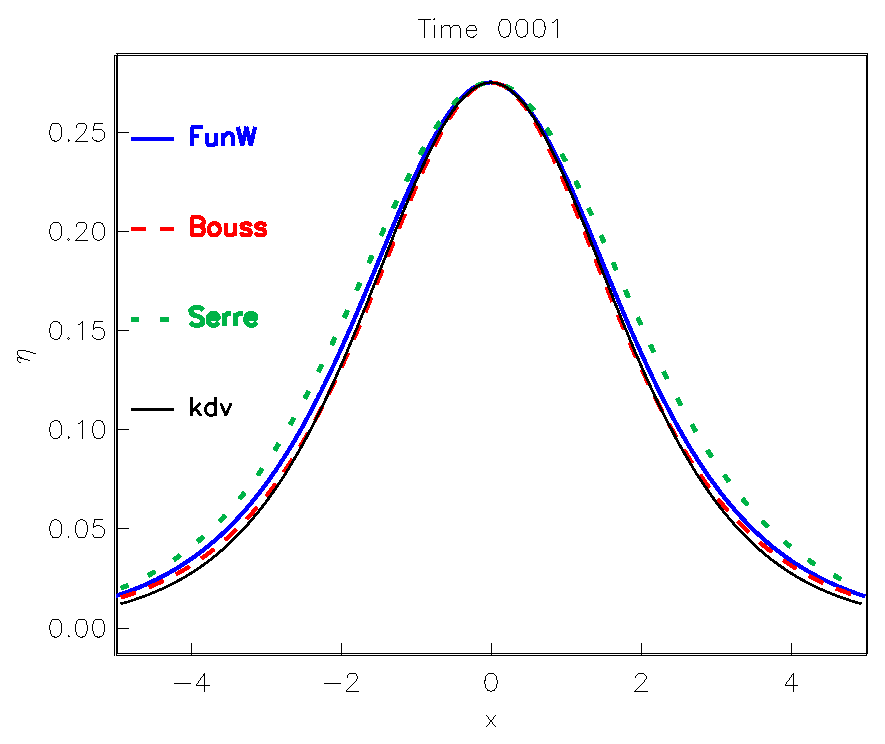
\includegraphics[width=111.55\unitlength,height= 93.00\unitlength]{FunSolA0001.ps}}
\put( 24.23,  3.50){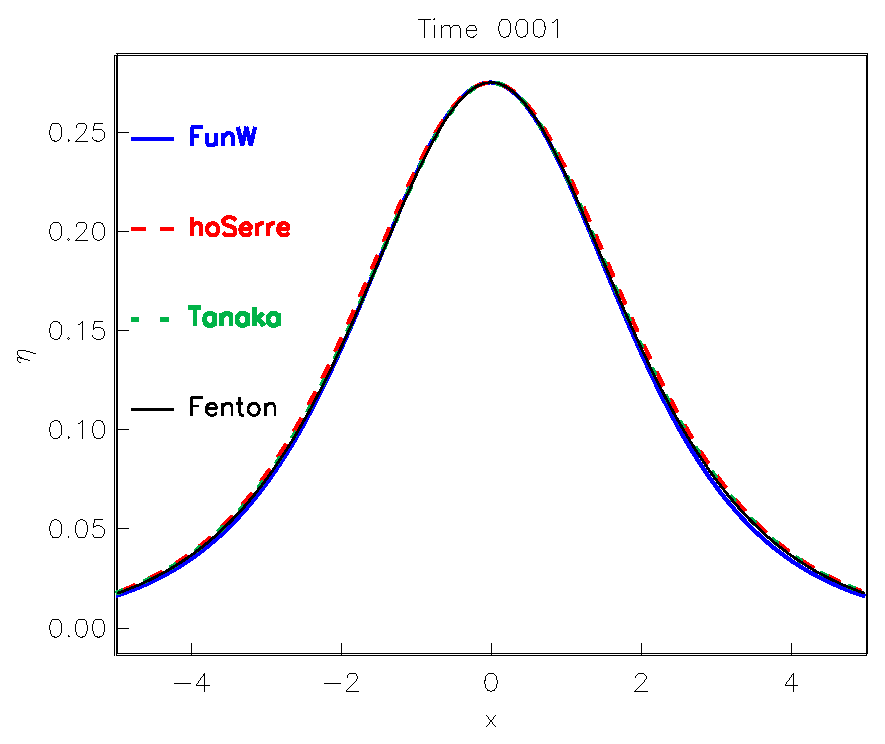
\includegraphics[width=111.55\unitlength,height= 93.00\unitlength]{FunSolB0001.ps}}
\end{picture}}
}
\caption[\ ]{ 
Funwave solutions and solitons}
\end{figure}
\begin{figure}
\centerline{
\makebox{
\setlength{\unitlength}{1mm}
\begin{picture}(160,200)
\put( 24.23,103.50){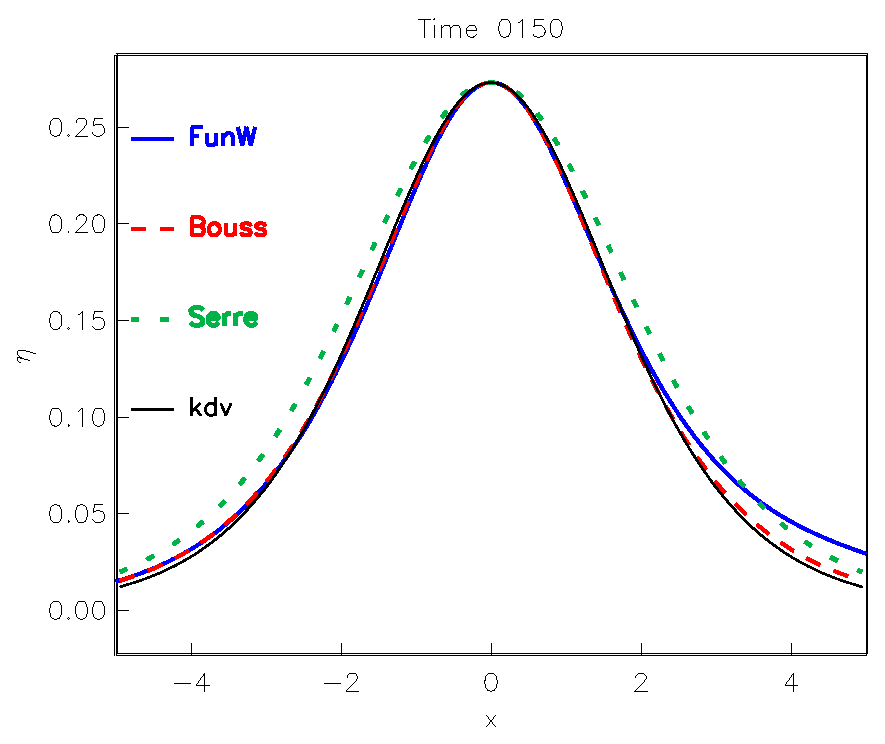
\includegraphics[width=111.55\unitlength,height= 93.00\unitlength]{FunSolA0150.ps}}
\put( 24.23,  3.50){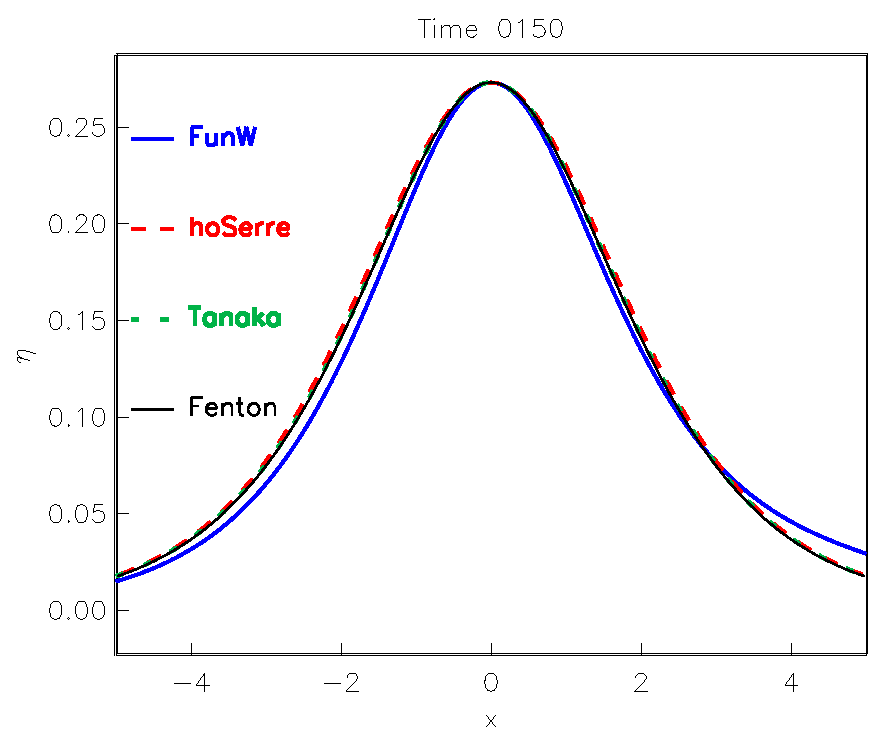
\includegraphics[width=111.55\unitlength,height= 93.00\unitlength]{FunSolB0150.ps}}
\end{picture}}
}
\caption[\ ]{ 
Funwave solutions and solitons}
\end{figure}
\begin{figure}
\centerline{
\makebox{
\setlength{\unitlength}{1mm}
\begin{picture}(160,200)
\put( 24.23,103.50){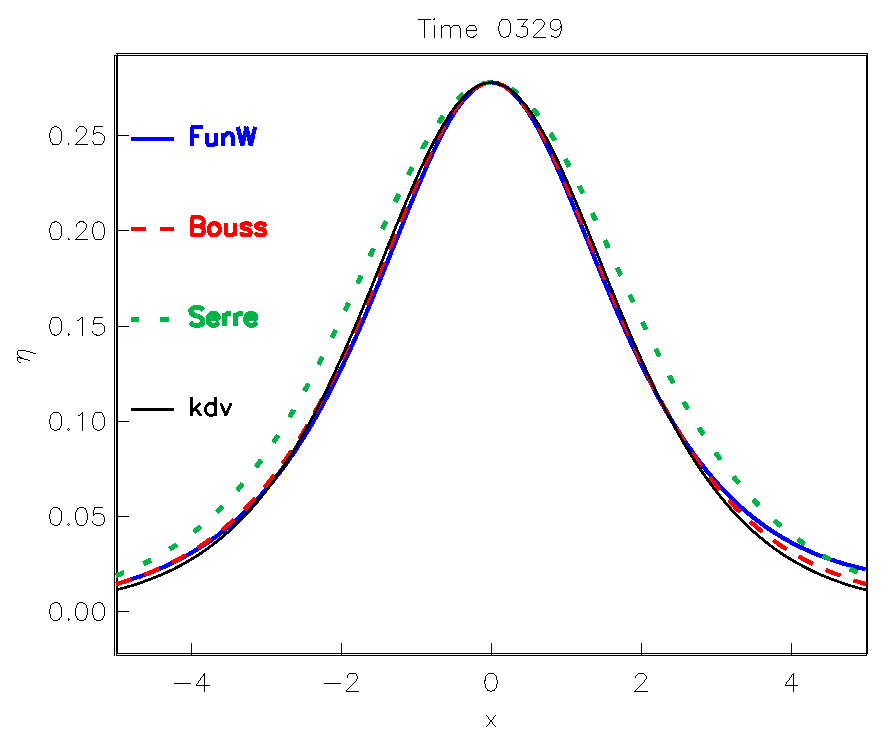
\includegraphics[width=111.55\unitlength,height= 93.00\unitlength]{FunSolA0329.ps}}
\put( 24.23,  3.50){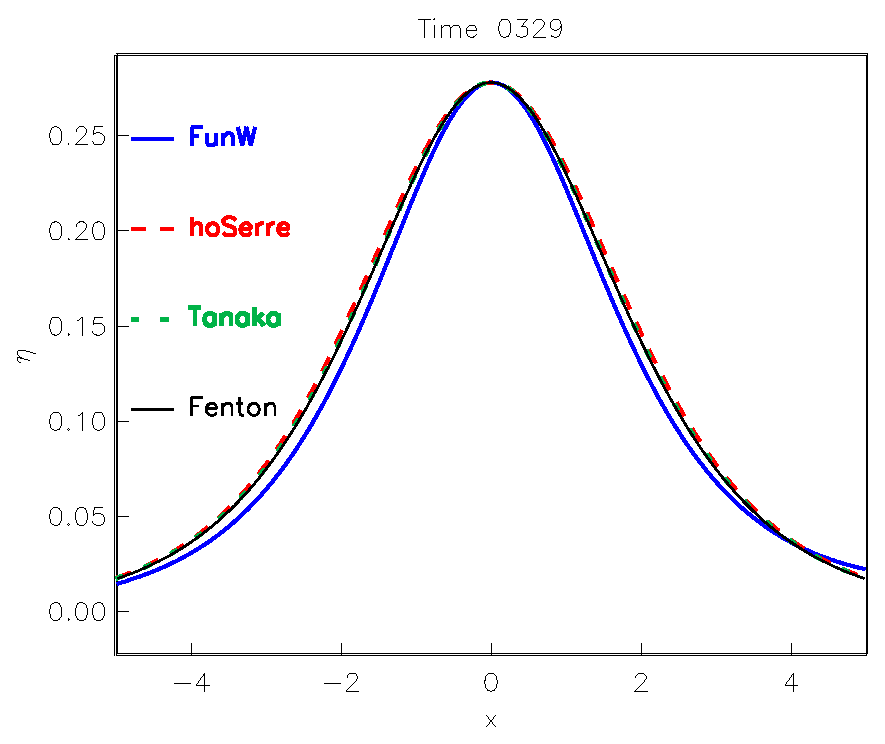
\includegraphics[width=111.55\unitlength,height= 93.00\unitlength]{FunSolB0329.ps}}
\end{picture}}
}
\caption[\ ]{ 
Funwave solutions and solitons}
\end{figure}
